 \documentclass[twoside,reqno,11pt]{article}

 \usepackage{algorithm,algorithmic} 

% to have 2-digits numbering for equation, use:
 \def\theequation{\arabic{section}.\arabic{equation}}

  \setcounter{page}{1}
  \thispagestyle{empty}

%%%%%%%%%%%%%%% begin make title %%%%%%%%%%%%%%

 %%% TITLE: texts in [.] is abbreviated (1st line) title for running heads
 %%% Author(s): put in brackets [.] the short author's name

 \title{AN EFFICIENT DEEP MEMORY ALGORITHM FOR COMPUTING FRACTIONAL ORDER OPERATORS} 
 \author{Steven Dorsher $^1$, Gary Bohannan $^2$, Chad Bohannan $^3$}

%%%%%%%%%%%%%%%%%%%%%%%%%%%%%%%%%%%%%%%%%%%%%%%%%%%%%%%%%%%%%%%%%%%%%%%
                    % THE BEGINNING %
 \begin{document}

\maketitle

%%%% Abstract %%%%%%%%%%%%%%%%%%%%%%%%%
 \begin{abstract}

This paper outlines a method to achieve effective bandwidth of five or
more decades in the approximation of a fractional order
derivative. This constitutes an increase of two decades or more over
current algorithms, such the Infinite Impulse Response (IIR) method
based on continued fraction expansion, while demanding only slightly
more computational steps and processor memory.

 \medskip

%{\bf Do these sound right? Same with the keywords I chose below}
%{\it MSC 2010\/}: Primary 65Y02: Secondary 65Z02, 65Y04, 65Z04

 \smallskip

{\it Key Words and Phrases}: digital fractors, memory kernel,
fractional calculus, numerical methods, computational efficiency

\end{abstract}


%%%%%%% end make title %%%%%%%%%%%%%%%%%%%%%%%%%%%%%%%%%%
 \vspace*{-16pt}

%%%%%%%% begin papers' body %%%%%%%%%%%%%%%%%%%%%%%%%%%%%

\section{Introduction}\label{sec:intro}
\setcounter{section}{1}
\setcounter{equation}{0}

Interest in the application of the fractional calculus has been
growing at an ever increasing rate. Of long term and continued
interest is in the use of fractional order (FO) operators, such as
integrators and differentiators, in motion control
applications.~\cite{Luo:13} While wide bandwidth analog controllers
have been successfully demonstrated~\cite{Bohannan:08}, fractional
order analog circuit elements are not generally available and the
prototypes that have been demonstrated do not have the ability to be
retuned for a specific desired phase.~\cite{Monje:10}

Unfortunately, the existing techniques for digital approximation of FO
operators are limited in bandwidth to on the order of three and a half
decades of frequency response while nonlinear effects in motion
control systems can span five decades or more. This places a severe
constraint on the design and implementation of digital FO controllers,
i.e. how to set the sampling frequency to meet the high speed
requirements necessitated by the Nyquist sampling rate while at the
same time providing enough deep memory to get low offset
error. Additionally, the infinite impulse response type of
implementation cannot guarantee stability due to the limitations of
finite precision arithmetic. See e.g.~\cite{Chen:04a}.

Given the current necessity to implement FO controls in digital form,
it is desirable to obtain the most efficient algorithm to compute a
fractional order operator while maximizing the numerical stability of
the algorithm. Efficiency to be measured in both memory utilization
and number of computations per time step. This paper outlines a
computational method inspired by the Riemann-Liouville integral
definition and the Gr{\"u}nwald algorithm.~\cite{OldSpan:74} The
essential concept is the rescaling of time by successive accumulation
of older data into increasing size bins for deeper memory.




\paragraph{Outline\\}
We will first briefly describe the current state of the art in
fractional order operator approximation and then describe a novel
approach based on successive binning of older data.

\begin{itemize} 
\item Section~\ref{sec:algorithmDefn} will contain algorithm definitions. 
\item Section~\ref{sec:bode} will contain the amplitude and phase response
  of these algorithms for a large and small number of bins in the
  partition.
\item Section~\ref{sec:computation} will contain an analysis of the
  computational resources required for the larger versus the smaller
  number of memory registers stored.
\end{itemize}

%%%%%%%%%%%

\section{Algorithm definitions}\label{sec:algorithmDefn}
\setcounter{section}{2}
\setcounter{equation}{0}

\vspace{-12pt}
\subsection{Partitioning the Grunwald history into averaged bins}\label{subsec:avgShift}
The technology most widely used today in digital fractional order
circuitry is the continued fraction expansion (CFE) approximation to
$s^\alpha$. Its benefits are that it was a flat phase response over
approximately two and a half decades in phase for a 9th order
expansion (10 registers of input signal memory). It would be desirable
to find an algorithm with an even broader flat phase frequency
bandwidth and with a comparably small amount of memory required. We
take the Grunwald algorithm as a starting point. As the signal history
retained in the Grunwald sum grows longer, the bandwidth of flat phase
response grows broader; however, the memory required also increases
with input signal history length. To reduce this memory requirement
and retain a long signal history, we propose partitioning the input
signal history into bins that are longer further into the past. The
value of the binned input signal is represented by the average value
of the input signal within that bin. The presence of short bins at
recent times maintains sensitivity to high frequencies, while the
inclusion of long bins at past times adds sensitivity to low
frequencies that would not usually be present in a Grunwald sum with
the same number of terms. (See Figure~\ref{fig:freqScaling}).

\begin{figure}
\epsfig{file=sensitivityIsFreqDependent.eps, height=1.5in, width=4in}
\label{fig:freqScaling}
\caption{Let each division represent a single time step and each bar represent a bin, scaled such that the duration of a bin increases further back in time (toward the right). The value of the bin is the average of the input signal, the sine wave, at each point in time within that bin. There exists some oldest bin that responds sensitively to the input signal (in this figure, the second bin). For lower frequencies, that oldest bin moves to older times. This illustrates the sensitivity of short bins at recent times to high frequencies and long bins in the distant past to low frequencies.}
\end{figure}


\subsection{Modified Grunwald}

The Grunwald form of the fractional integral can be written~\cite{OldSpan:74}

\begin{equation}
_0D^\alpha_tf(t) = \displaystyle \lim_{N\to\infty} \left(\frac{t}{N_t}\right)^{-\alpha}
\displaystyle\sum\limits_{j=0}^{N_t-1} w_{j}x_j
\label{simpleGrunwald}
\end{equation}
where $f(t)$ is the input signal at time $t$, the $j$th value of the
input signal history is $x_j=f\left(t-\frac{j\Delta t}{N_t}\right)$, and the
$j$th Grunwald weight is

\begin{equation}
w_{j} = \frac{\Gamma(j-\alpha)}{\Gamma(j+1)\Gamma(-\alpha)}.
\label{wj}
\end{equation}
To include more distant history at low computational cost, we modify
the Grunwald sum of Equation~\ref{simpleGrunwald} by partitioning its
history into $N_b$ bins. In each bin $k$, the input signal history
$x_j$ is represented by its average value over that bin, $X_k$.

Since we make the assumption that each value is well represented by
its average within a bin, we can define a value for the "bin
coefficient" by summing the Grunwald coefficients within that bin.

\begin{equation}
W_k = \displaystyle\sum\limits_{j=p_{k-1}+1}^{p_k} w_j
\label{eqn:sumWk}
\end{equation}

\noindent where $w_j$ is summed from the lowest index of the input data history within bin $k$ to the highest index $p_k$ within that bin. There is an additional factor that goes into $\bar{W}$ that will be discussed in Section~\ref{sec:shifting}. 

With these definitions, the modified Grunwald differ-integral can be written

\begin{equation}
_0D^\alpha_t f(t) = \displaystyle(\Delta t)^{-\alpha}\sum\limits_{k=0}^{N_b}\bar{W}_kX_k
\label{avgSimpleGrunwald}
\end{equation}
where $\Delta t$ is the interval between time samples.



\subsection{Updating the average history}
\label{sec:shifting}

When a new input data element is read, the history is updated. The new data element is shifted into the first bin through a weighted average. Since data elements represent time steps, they should be incompressible-- when one element is shifted into a bin, another virtual element should be shifted out of that bin if the bin is full. It shifts into the next bin, and pushes a virtual element out of that one, until a bin which is partially full or empty is reached. To update the average data stored in the bins, we take the weighted average obtained by adding one virtual element from the $(k-1)$th bin to the $b_k$ elements in the $k$th bin. This process is illustrated in Figure~\ref{fig:binShifting}.

\begin{figure}
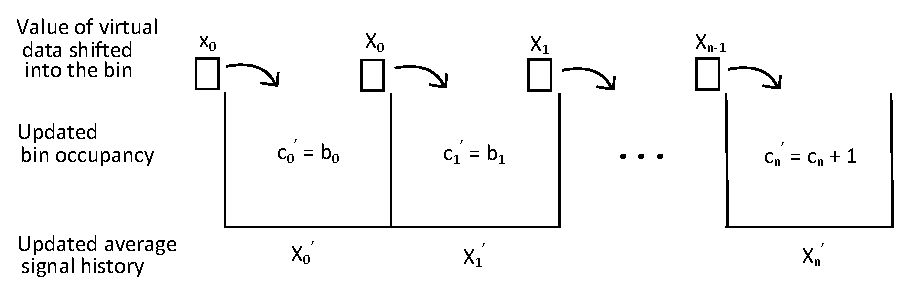
\epsfig{file=binShifting.eps,height=2in,width=5in}
\label{fig:binShifting}
\caption{When the input data $x_0$ is read, virtual data elements with bin average values $X_k$ are shifted from the $k$th to the $(k+1)$th bin. The first $n-1$ bins are at capacity, but the $n$th bin gains one data point. The bin averages are updated to value $X_k^\prime$ through a weighted average.}
\end{figure}

During start-up, it will be necessary to consider bins that have some
set size $b_k$, but are not filled to that capacity. In that case, it
is the current occupation number $c_k$ of each bin that enters the
calculation. If the $k$th bin initially contains $c_k$ elements,
updating the history either leaves $c_k$ ($c_k\prime=c_k=b_k$) or
increments the number of elements in the bin such that $c_k\prime =
c_k + 1$ if the bin is not yet at capacity. Either way, the updated
average of the value of the $k$th bin, $X_k\prime$, is given by

\begin{equation}
X_k^\prime = \frac{c_k^\prime-1}{c_k^\prime}X_k + \frac{1}{c_k^\prime}X_{k-1}.
\label{eqn:updating}
\end{equation}
where $X_{-1}$ is taken to be $x_0$, the input data that has just been
read. 

During start-up, these partially full bins may also factor into
the Grunwald weights. To handle bins that are partially full, we
weight the binned Grunwald weights by the ratio of the bin occupation
number $c_k$ to its capacity $b_k$,

\begin{equation}
\bar{W}_k= \frac{c_k W_k}{b_k}.
\label{eqn:Wbar}
\end{equation} 











%%%%%%%%%%%%%%%%%%%%%

\section{Amplitude and phase characteristics}\label{sec:bode}
\setcounter{section}{3}
\setcounter{equation}{0}

%%%%%%%%%%%%

\section{Analysis of computational resources}\label{sec:computation}
\setcounter{section}{4}
\setcounter{equation}{0}

The computational efficiency of each algorithm concerns both the
memory used by the algorithm and the number of computational steps
required for the algorithm to execute, which is a measure of the
speed. To characterize the operational efficiency of a digital fractor
operating as a circuit element in real time, the quantities of
interest are the memory or number of processor steps {/em per time
  step}.

\vspace{-12pt}
\subsection{The average Grunwald algorithm}
To count the number of processor steps required, the algorithms
described in Section~\ref{subsec:avgShift} are converted to pseudocode
then the conversions listed in Table~\ref{tab:stepCounting} are
applied.

\begin{table}
\begin{tabular}{ll}
\hline
Type    &Cost   \\
\hline
Integer assign  &Free\\
Floating point assign &Free \\
Negation &Free \\
Integer $+$,$-$ &Free \\
Floating point $+$,$-$ &1 \\
Integer $*$,$\/$ &1 \\
Floating point $*$,$\/$ &1 \\
Floating point exponentiation &1 \\
If (int clause) &Free \\
If (float clause) &1 \\
While (int clause) &1 \\
While (float clause) &2 \\
\hline
\end{tabular}
\label{tab:stepsCounting}
\caption{Number of processor steps required for various operations.}
\end{table}

During intialization, several things must happen. The array defining
the binning structure, $b_k$, must be set. The history of the input
signal must be zeroed and the first output must be set to zero as
well. Most significantly, the binned weights must be calculated for
the chosen binning structure.

The time it takes to calculate or set $b_k$ is moderately dependent
upon the details of the binning structure chosen. However, any binning
structure will have a processing time that scales as $N_b$ rather than
$N_t$ because of the number of bins that must be set. Here $N_t$ is
the maximum history depth in time-steps of the $N_b$ memory storage
bins. By definition,

\begin{equation}
N_t = \displaystyle\sum_{k=0}^{N_b}b_k.
\label{eqn:Nt}
\end{equation}

Since zeroing (assignment) is computationally free, the bulk of the
initialization process occurs during the computation of the
weights. Since each individual Grunwald weight must be summed, this
process scales as $N_t$. Equation~\ref{eqn:Wk} gives the algorithm for
the calculation of the bin weights. The following recursion formula
for Grunwald weights can be used to iterate $w_j$ to a new value with
each time step. In the $j$th time step, $w_j$ has the value

\begin{equation}
w_j = \frac{j-1-\alpha}{j}w_{j-1}.
\label{eqn:GrunwaldRecursion}
\end{equation}

In the implementation of an algorithm for initialization of the
weights, individual Grunwald weights $w_j$ need not be stored in an
array after calculation. These individual weights can be summed
immediately into the corresponding bin weights $W_k$ according to
Equation~\ref{eqn:sumWk}, at which time the value of $w_j$ may be safely
overwritten with $w_{j+1}$.

Using these formulas, pseudocode for the weight-initialization
algorithm is given in Algorithm~\ref{alg:initializing}.

\begin{algorithm}
\caption{Initialization of the binned weights. $\alpha$ is the order of the differintegral and $b_k$ is the bin capacity of the $k$th bin.}
\label{alg:initializing}
\begin{algorithmic}
%\REQUIRE $0 \le \alpha \le 1$
%\ENSURE Equation~\ref{eq:Wk}
\FOR{$0\le k < N_b$}
\STATE $W_k \gets 0.0$
\ENDFOR
\STATE $j \gets 1$
\STATE $k \gets 0$
\STATE $w \gets 1.0$
\STATE $p \gets b_0$
\WHILE{$k < Nb$}
\STATE $W_k \gets W_k + w$
\STATE $j \gets j +1$
\IF{$j>p$}
\STATE $k \gets k +1$
\STATE $p \gets p +b_k$
\ENDIF
\STATE $w \gets \frac{j-1.0-\alpha}{j}w$
\ENDWHILE
\end{algorithmic}
\end{algorithm}
Using Table~\ref{tab:stepsCounting}, the number of processor steps
required to implement the weight initialization algorithm is $5N_t+1$.

\smallskip

Equation~\ref{eqn:updating} may be used as the basis for an algorithm
to update the binned average input signal history values when a new
input signal value is read. Care must be taken to account for the
filling of the bins until the approximation reaches steady-state.

Again, a memory saving opportunity is available. Since only one bin
can be filling at a time and the rest must be either full ($c_k=b_k$)
or empty ($c_k=0$), the full array of $N_b$ occupancy numbers $c_k$
need not be stored. Instead, it is sufficient to store the index of
the bin that is filling, $k_{filling}$ and its occupancy,
$c_{filling}$. These unfilled bins with $k>k_{filling}$ and $c_k=0$
are not updated when a new input signal value is read into the
history.

Pseudocode for the bin-average updating algorithm is given in
Algorithm~\ref{alg:updating}.

\begin{algorithm}
\caption{Algorithm for updating the bin average values of the input signal history. $X_{k}$ is the $k$th average binned value of the history. $x_0$ is the input signal value that has just been read into the digital fractor.}
\label{alg:updating}
\begin{algorithmic}
%\STATE $k_{filling}\gets 0$
%\STATE $c_{filling}\gets 0$
\STATE $k \gets N_b$
\WHILE{$k>0$}
\IF{$k=k_{filling}$}
\STATE $c_{filling}\gets c_{filling} +1$
\IF{$c_{filling}>b_k$}
\STATE $k_{filling} \gets k_{filling} +1$
\ENDIF
\STATE $k\gets k+1$
\STATE $X_k \gets \left(1.0-\frac{1.0}{c_{filling}}\right)X_k 
- \frac{1.0}{c_{filling}}X_{k-1}$
\ELSIF{$k<k_{filling}$}
\STATE $X_k \gets \left(1.0-\frac{1.0}{b_k}\right)X_k 
- \frac{1.0}{b_k}X_{k-1}$
\ENDIF
\STATE $k\gets k -1$
\ENDWHILE
\IF{$k_{filling}=0$}
\STATE $c_{filling} \gets c_{filling} +1$
\IF{$c_{filling}>b_0$}
\STATE $k_{filling} \gets 1$
\STATE $c_{filling} \gets 1$
\ENDIF
\STATE $X_k \gets \left(1.0-\frac{1.0}{c_{filling}}\right)X_0 
- \frac{1.0}{c_{filling}}x_{0}$
\ELSE
\STATE $X_k \gets \left(1.0-\frac{1.0}{b_0}\right)X_0 
- \frac{1.0}{b_0}x_{0}$
\ENDIF
\end{algorithmic}
\end{algorithm}
Table~\ref{tab:stepsCounting} yields $12N_b$ processor steps
required to update the bin average values of the input signal history
when a new data point is read.

\smallskip

Our algorithm for differintegration is based upon
Equations~\ref{eqn:avgSimpleGrunwald}~and~\ref{eqn:Wbar}. The
algorithm is shown in Algorithm~\ref{alg:modGrun}.

\begin{algorithm}
\caption{The algorithm for differintegration using the modified Grunwald method described in Section~\ref{sec:avgShift}}.
\label{alg:modGrun}
\begin{algorithmic}
\STATE $k\gets N_b$
\WHILE{$k\ge 0$}
\IF{$k=k_{filling}$}
\STATE $W_k\gets\frac{c_{filling}}{b_k}W_k$
\ENDIF
\STATE $D_t^\alpha \gets D_t^\alpha + W_kX_k$
\ENDWHILE
\STATE $D_t^\alpha \gets (\Delta t)^{-\alpha}D_t^\alpha$
\end{algorithmic}
\end{algorithm}
Based upon Table~\ref{tab:stepsCounting}, the number of processor
steps required to calculate the differintegral using the modified
Grunwald approach presented in this paper is $3N_b+2$.

\begin{table}
\begin{tabular}{ll}
\hline
Stage &Processor steps required \\
\hline
Initialization of weights &$5N_t+1$ \\
Updating the average bin history values &$12N_b$ \\
Summing the differintegral &$3N_b+2$\\
\hline
\end{tabular}
\caption{Processor steps required for the different stages of the average Grunwald algorithm.}
\label{tab:processor}
\end{table}

\smallskip

The number of processor steps required for the three stages are
summarized in Table~\ref{tab:processor}. Memory requirements for the
algorithms described in this section are shown in
Table~\ref{tab:memory}. 

The two real-time operation stages, updating and differintegrating,
together require $15N_b+2$ processor steps. With 26 bins ($N_b=26$),
$392$ processor steps are required for each time-step of a fractional
order differentiation or integration. $3N_b+6=84$ memory registers are
required for 26 bins of history.

Initialization, on the other hand, is a very resource-consuming
process. For an exponentially scaled binning structure with a scale
factor of two, $N_t=2^{26}-1=67,108,863$ for 26 bins. Initialization
therefore requires $3.36\times 10^8$ processor steps, a calculation
perhaps best achieved by a computer in a one-time operation. 


\begin{table}[h]
\begin{tabular}{llll}
\hline
Variable& Definition & Size& Stages \\
\hline
$b_k$ & Bin capacity & $N_b$ &I, U, D \\
$W_k$ & Binned weights & $N_b$ &I, U, D \\
$X_k$ & Binned history & $N_b$ &I, U, D \\
$x_0$ & Current input data & 1 & U \\
$D_t^\alpha$ & Output differintegral & 1 & I, D\\
$\alpha$ &Order of differintegral &1 &I, D\\
$N_b$ &Number of bins &1 &I,U,D\\
$N_t$ &Number of time steps stored &1 & I\\
$\Delta t$ &Time step &1 &D\\
$w_j$ & Grunwald weight, temp variable & 1 & I\\
$k_{filling}$ & Currently filling bin & 1 & U, D\\
$c_{filling}$ & Occupancy of filling bin & 1 & U, D \\  
\hline
\hline
& Total w/o initialization &$3N_b+6$ &\\
 & Total & $3N_b+9$ &\\
\hline
\end{tabular}
\label{tab:memory}
\caption{Accounting for memory in the Average-Shift algorithm. I = Initialization, U=Updating, D = Differintegration}
\end{table}




%%%%%%%%%%%%%%%%

\section{Conclusions}\label{conclusions}
\setcounter{section}{5}
\setcounter{equation}{0}

%%%%%%%%%%%%%%%


%%%%%%%%%%%%%%%%%%%%%%%%%%%%%%%%%%%%%%%%%%%%%%%

\smallskip
%%%%%%%%%%%%%%%%%%%%%%%%%%%%%%%%%%%%%%%%%%%%%%%%%
\section*{Acknowledgements}

The author thanks his institution for the support, under Grant No
...

%%%%%%%%%% References %%%%%%%%%%%%%%%%%%%%%%%%%%%%%%%%
%%%% arranged in ALPHABETIC ORDER of Authors' Families

%%%%%%%%%% References %%%%%%%%%%%%%%%%%%%%%%%%%%%%%%%%
%%%% arranged in ALPHABETIC ORDER of Authors' Families

 \begin{thebibliography}{99}
 \normalsize

\bibitem{Bohannan:08}
  G. Bohannan,
  Analog Fractional Order Controller in Temperature and Motor Control Applications.
  {\it Journal of Vibration and Control} {\bf 14(9-10)} (2008), 1487-1498.



\bibitem{Chen:04a}
  Y. Chen, B. Vinagre, I. Podlubny,
  Continued fraction expansion approaches to discretizing fractional order
    derivatives -- an expository review.
  {\it Nonlinear dynamics}. {\bf 38} (2004), 155-170.


\bibitem{Luo:13}
  Y. Luo, Y. Chen,
  {\it Fractional Order Motion Controls}.
  John Wiley {\&} Sons, Chichester, West Sussex (2013).

\bibitem{Monje:10}
  C. Monje, Y. Chen, B. Vinagre, D. Xue, V. Feliu,
  {\it Fractional-order Systems and Controls: Fundamentals and Applications, a monograph in the Advances in Industrial Control Series}.
  Springer, Berlin (2010).


\bibitem{OldSpan:74}
  K. Oldham, J. Spanier,
  {\it The Fractional Calculus}.
  Academic Press, New York (1974). 

\end{thebibliography}



%%%%%%%%%% put authors' addresses here, in \it %%%%%%%%%%%%

\bigskip \smallskip


\it
% (First) Author's full postal address
$^1$ Department of Physics \\
St Cloud State University \\
mailing address: 3152 Blackheath Drive \\
Saint Cloud, MN 56301, USA \\ [4pt]
email: sdorsher@gmail.com

\hfill Recieved: ???

%Second author's address
$^2$ Department of Physics\\
Saint Cloud State University\\
720 4th Avenue South\\
Saint Cloud, MN 56301, USA\\ [4pt]
email: gwbohannan@stcloudstate.edu

%Third author's address
$^3$ Chad Bohannan \\
email: chad.bohannan@gmail.com


\end{document} %%%%%%%%%%%%%%%%%%%%%%%%%

